%%%%%%%%%%%%%%%%%%%%%%%%%%%%%%%%%%%%%%%%%%%%%%%
%%% Template for lab reports used at STIMA
%%%%%%%%%%%%%%%%%%%%%%%%%%%%%%%%%%%%%%%%%%%%%%%

%%%%%%%%%%%%%%%%%%%%%%%%%%%%%% Sets the document class for the document
% Openany is added to remove the book style of starting every new chapter on an odd page (not needed for reports)\sceau{Pictures/sceauULB.jpg}
\documentclass[10pt,french, openany]{book}

%%%%%%%%%%%%%%%%%%%%%%%%%%%%%% Loading packages that alter the style

\usepackage[french]{babel}
\usepackage[]{graphicx}
\usepackage[]{color}
\usepackage{alltt}
\usepackage[T1]{fontenc}
\usepackage{amsmath}
\usepackage[utf8]{inputenc}
\usepackage{gensymb}
\usepackage{booktabs}
\usepackage{hyperref}
\usepackage{csquotes}
\usepackage{epstopdf}
\usepackage[section]{placeins}
\usepackage{wrapfig}
\usepackage{float}
\epstopdfDeclareGraphicsRule{.gif}{png}{.png}{convert gif:#1 png:\OutputFile}
\AppendGraphicsExtensions{.gif}
\usepackage[lofdepth,lotdepth]{subfig}

\usepackage[pages=some]{background}
\hypersetup{
    colorlinks=true,
    linkcolor=black,
    citecolor=black,
    filecolor=magenta,      
    urlcolor=cyan,
    pdftitle={Rapport de stage : Etude d'une étoile variable à courte période},
    pdfauthor={Louise Bizel \& Nicolas Grimbaum},
    }
\usepackage[backend=biber,style=numeric, sorting = nty, defernumbers=true]{biblatex}

\addbibresource{stage.bib}
\setcounter{secnumdepth}{3}
\setcounter{tocdepth}{3}
\setlength{\parskip}{\smallskipamount}

% Set page margins
\usepackage[top=100pt,bottom=100pt,left=68pt,right=66pt]{geometry}

% Package used for placeholder text
\usepackage{lipsum}

% Prevents LaTeX from filling out a page to the bottom
\raggedbottom

% Adding both languages

% All page numbers positioned at the bottom of the page
\usepackage{fancyhdr}
\fancyhf{} % clear all header and footers
\fancyfoot[C]{\thepage}
\renewcommand{\headrulewidth}{0pt} % remove the header rule
\pagestyle{fancy}

% Changes the style of chapter headings
\usepackage{titlesec}
\titleformat{\chapter}
   {\normalfont\LARGE\bfseries}{\thechapter.}{1em}{}
% Change distance between chapter header and text
\titlespacing{\chapter}{0pt}{50pt}{2\baselineskip}

% Adds table captions above the table per default
\usepackage{float}
\floatstyle{plaintop}
\restylefloat{table}

% Adds space between caption and table
\usepackage[tableposition=top]{caption}

% If multiple images are to be added, a folder (path) with all the images can be added here 
\graphicspath{ {Figures/} }

% Separates the first part of the report/thesis in Roman numerals
\frontmatter
\backgroundsetup{
scale=1,
color=black,
opacity=0.05,
angle=10,
position={12cm,-22cm},
contents={%
  
\includegraphics[height=20cm,width=20cm,keepaspectratio]{sceauULB.jpg}
  }%
  }
%pour des beau tableau à double ligne
\usepackage{hhline}


%%%%%%%%%%%%%%%%%%%%%%%%%%%%%% Starts the document
\begin{document}

%%% Selects the language to be used for the first couple of pages
\selectlanguage{french}

%%%%% Adds the title page
\begin{titlepage}
	\clearpage\thispagestyle{empty}
	\centering
	\vspace{1cm}
    \BgThispage

	% Titles
	% Information about the University
	{\normalsize Rapport de stage de BA-3 \\
		Institut d'Astronomie et d'Astrophysique \\
		Université Libre de Bruxelles \par}
		\vspace{3cm}
	{\Huge \textbf{Etude de l'étoile variable DU Boo}} \\
	%\vspace{1cm}
	%{\large \textbf{xxxxx} \par}
	\vspace{4cm}
	{\normalsize Louise BIZEL \\ % \\ specifies a new line
	             Nicolas GRIMBAUM\par}
	\vspace{5cm}
    
    \centering 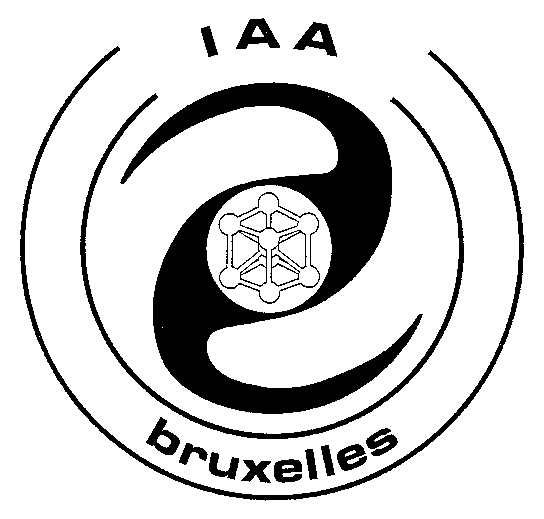
\includegraphics[scale=0.2]{iaa_home_logo.png}
    
    \vspace{0.5cm}
		
	% Set the date
	{\normalsize \today \par}
	
	\pagebreak

\end{titlepage}

% Adds a table of contents
\tableofcontents{}
\BgThispage
%%%%%%%%%%%%%%%%%%%%%%%%%%%%%%%%%%%%%%%%%%%%%%%%%%%%%%%%%%%%%%%%%%%%%%%%%%%%%%%%%%%%%%%%%%%%
%%%%%%%%%%%%%%%%%%%%%%%%%%%%%%%%%%%%%%%%%%%%%%%%%%%%%%%%%%%%%%%%%%%%%%%%%%%%%%%%%%%%%%%%%%%%
%%%%% Text body starts here!
\mainmatter

\chapter{Introduction}\label{chapt:sum}

La définition d'une étoile variable peut être assez général comme toute les étoiles évoluent dans le temps. Mais certaines ont une luminosité variable sur de courte durée ou varie périodiquement résultant de pulsation de leur couche externe. La classification de ces étoiles fut très tôt l'intérêt des sociétés d'astronomes. En effet,les traces que nous avons de l'observation des étoiles variables remonte à des papyrus égyptien du 10e siècle avant notre ère. Aujourd'hui, il existe des catalogues très complet détaillant les caractéristiques de variations de nombreuses étoiles. Ces observations permettent de comprendre les principes régissant l'équilibre des étoiles ainsi que leur évolution au cours de leur vie.

Dans le cadre d'un stage au département d'astronomie et d'astrophysique à l'université de l'ULB nous réalisons ce document présentant notre démarche et les données que nous avons obtenues lors de l'observation d'une étoiles variable sur une courte période. L'étoile variable choisie est déjà très bien décrite dans la littérature et notre but est de retrouver sa courbe de luminosité par nos propres observations. Nous utilisons pour ces observations les télescopes commandables à distance de l'entreprise ITelescope. Comme la location de ces télescopes à un prix, il est important de commencer par une étude préliminaire rigoureuse pour s'assurer de la nature de notre étoiles et des bonnes conditions de sa visibilité. Ensuite, après la validation de la part de nos promoteurs de stage, les prise de mesure sont programmer et les clichés renvoyé par ITelescope sont exploiter pour déterminer la luminosité de l'étoile à chaque phase observer et reconstruire ainsi sa variation de luminosité sur toute sa période.

\chapter{Travail préliminaire}
\section{Sélection du télescope}

    Tout d'abord, nous devons choisir le télescope que nous allons utiliser pour observer l'étoile variable, parmi ceux mis à disposition par iTelescope. Il faut cependant respecter les contraintes suivantes :
    
    \begin{itemize}
        \item Diamètre compris entre 15 et 35 cm
        \item Monté d'un filtre Johnson/Cousin V
        \item Full well du CCD\footnote{Charge Couple Device} le plus grand possible
        \item Sans anti-blooming
    \end{itemize}
    
    Le diamètre du télescope est un facteur limitant pour l'observation d'étoiles de petites magnitudes. Un diamètre supérieur à 15 cm permet de se placer à une magnitude limite d'environ 13,6 \cite{Griffiths0}. La taille du télescope est aussi limitée par le coût de ce dernier. Les télescopes plus larges sont plus chers. N'ayant besoin d'un télescope de diamètre très grand pour les magnitudes des étoiles que nous observerons, il est donc d'autant plus intéressant de se restreindre à une classe de télescopes de petite dimension.
    
    Les télescopes sont équipés de capteurs CCD qui ne capturent des images qu'en nuances de gris. Bien sûr, il existe de nombreux appareils photographiques ou vidéo qui sont capables d'enregistrer en couleurs. Les pixels des capteurs de ces appareils sont groupés par trois, et chacun des pixels appartenant à un groupe est sensible à une couleur (rouge, vert ou bleu), et l'image en couleur est ensuite reconstruite à partir de ces informations. Il en résulte que l'implémentation des couleurs sur ces appareils se fait au détriment de la résolution. Une autre approche pour les caméras vidéos est de combiner trois capteurs CCD et un jeu de filtres pour séparer la lumière incidentes selon les couleurs. L'image peut alors être reconstruite en couleurs sans perte de résolution.Cependant ces techniques fonctionnent assez bien pour des modes vidéos normaux où l'exposition est très courte, mais pour une pratique astronomique où l'exposition est plus grande (généralement en secondes ou en minutes) car la lumière est rare, il est important d'utiliser le maximum de lumière incidente et de pixels disponibles sur le capteur.
    Ainsi, la façon la plus optimale d'enregistrer des images dans ce contexte est d'utiliser l'entièreté des pixels pour capturer la lumière incidente. Si l'on souhaite effectuer une image en couleurs, on doit donc prendre autant de clichés que l'on a de filtres nécessaires pour recomposer les couleurs.\cite{Griffiths0, manual:sbig}
   
    Dans notre cas, le seul filtre qui nous intéresse est le filtre V (pour Visual) du système photométrique UBVRI, dont la bande passante est centrée autour de 550nm, correspondant donc à la sensibilité de notre oeil, centrée dans la gamme du vert. En effet, cette gamme de lumière permet de simuler au mieux la réponse de l'oeil humain dans son interprétation de la luminosité, car celle-ci correspond à la gamme du visible \cite{cite:griffiths1, site:nsofiltre0, site:nsofiltre1}. Il s'agit avant tout d'un filtre dérivant d'un standard photométrique définissant la magnitude V depuis les années 1950 et jusqu'à nos jours dans le système UBV, mais aussi les systèmes de Genêve, Walraven et de Vilnius dans lesquels la longueur d'onde centrale diffère toutefois légèrement.\cite{book:landolt} Le 0 de magnitude V est définit dans le système UBV à partir de 6 étoiles de type A0V par Johnson\cite{article:johnson}. Ce système a par la suite été étendu par Cousins avec les filtres R et I et les filtres adaptés aux capteurs CCD développés par Bessell  \cite{article:cousin, article:bessell}. On appelle plus couramment la magnitude V comme la magnitude apparente, car correspondant à celle observée par l'oeil humain.
    
    Le full well d'un capteur CCD caractérise la quantité de charge que chaque pixel peut accumuler avant saturation. Une fois le pixel saturé, les charges reçues vont être perdues ou fuir vers les pixels adjacents. Ainsi, plus le full well est grand, plus on peut augmenter le temps d'exposition de l'image sans saturer le pixel. On améliore ainsi le rapport signal sur bruit en minimisant la perte d'information. \cite{manual:sbig, inbook:warner:CCD}
    
    Lorsqu'un pixel est saturé, les charges incidentes réparties sur les pixels voisins vont causer des trainées lumineuses verticales sur l'image. C'est ce que l'on appelle le blooming. Les capteurs équipés d'anti-blooming vont drainer les charges en excès du pixel, afin d'éviter cet effet, ce qui peut être intéressant si l'on souhaite effectuer une belle photographie d'une nébuleuse, sans pour autant observer des stries partant d'étoiles présentes dans le cadre. Comme l'on souhaite mesurer la quantité de charges incidentes, et que notre étude n'est pas à des fins esthétiques, il est préférable de ne pas disposer de cette fonctionnalité, afin de ne pas fausser les mesures. En effet, équippé d'anti-blooming, la réponse d'un pixel ne sera plus linéaire, et ne représentera donc plus la quantité de photons incidents. Le drain s'active en général lorsqu'un pixel est à 50\% de saturation. De plus la fabrication des capteurs anti-blooming implique une efficacité moindre d'environ 30\%. \cite{manual:sbig, inbook:warner:CCD}
    
    Il n'y a que deux télescopes qui respectent les conditions pré-citées, le T5 et le T18 \cite{site:T5, site:T18}. Dans un premier temps, nous choisissons de faire nos observations à l'aide du T18 car le T5 semble être plus prisé, et donc potentiellement moins disponible \cite{site:T5}. Par ailleurs, un autre groupe travaillant aussi sur l'étude d'une étoile variable à courte période a déjà choisi le T5, et il nous semble intéressant d'utiliser l'autre télescope. Cependant, pour des raisons pratiques, il a été convenu d'utiliser finalement le T5.  Comme les deux observatoires sont à des latitudes voisines, le changement du choix de télescope n'influera pas sur la visibilité de l'étoile que nous choisissons.
    
\pagebreak
\section{Sélection de la cible}
    Maintenant que nous avons sélectionné un télescope adéquat, nous pouvons utiliser ses coordonnées pour choisir l'étoile variable que nous allons étudier. Elle doit aussi respecter certaines contraintes :
    
    \begin{itemize}
        \item Magnitude V de minimum 11
        \item Variation de magnitude supérieur à 0.5 pour le minimum principal (0.3 pour l'éventuel minimum secondaire)
        \item Période de moins de 2 jour
        \item Visible par notre télescope de fin-février à mi-avril
        \item Présence d'étoiles de comparaison voisines de la cible
    \end{itemize}
    
    Il nous faut une étoile suffisamment visible compte tenu du diamètre du télescope T5 (250mm) et qui se distingue assez du bruit lumineux que nous aurons sur les clichés. La variation de sa magnitude doit être suffisamment marquée pour pouvoir la mesurer avec une erreur raisonnable. 

    Il nous est nécessaire d'étudier une étoile d'une période relativement petite. Comme nous voulons étendre nos prise de données sur un peu plus d'un mois, l'étoile doit être visible dans toute les phases, que nous sélectionnerons par la suite, à suffisamment d'occasion pour que nous puissions reconstruire un graphique exhaustif de la variation de sa magnitude sur une période. D'autant plus que le télescope T5 est assez utilisé, il nous faut donc prévoir que certaines observations prévues devront être reportées à plus tard car le télescope ne sera pas libre. La période doit aussi être assez différente d'un multiple de 24h. En effet dans le cas contraire les phases observables pendant la nuit seront toujours les même durant le mois où nous utiliserons le télescope et nous ne pourrions pas reconstruire sa période au complet.
    
    Comme notre télescope T5 se trouve au Nouveau Mexique nous pouvons déjà sélectionner les différentes constellation où notre cible pourrait être. La constellation doit se trouver dans l'hémisphère nord et doit être visible pendant le printemps. Ces critères nous permettent d'obtenir une liste de constellations candidates sur les 88 répertoriée.\cite{site:wiki:constellation}. Nous pouvons à présent utiliser un catalogue des étoiles variables pour y rentrer toutes nos contraintes et sélectionner notre cible. Le catalogue utilisé est le 'General Catalogue of Variable Stars' que l'on peut trouver sur Vizier \cite{site:vizier}. Le critère concernant l'hémisphère nord peut enfaîte être directement implémenté dans notre recherche dans le catalogue. Le T5 se situant à une latitude de 32$^{\circ}$N, l'étoile cible doit avoir une déclinaison comprise entre 15$^{\circ}$N et 45$^{\circ}$N. Ainsi nous obtenons une liste d'étoiles répondant à nos critères et nous pouvons choisir arbitrairement parmi les étoiles contenues dans les constellations visibles au printemps. Notre choix est tout de même guidé par la minimisation des erreurs venant du bruit. Il est donc intéressant de choisir une étoiles des plus lumineuse et avec une grande variabilité.
    
    L'étoile variable choisie est V*DU de la constellation du Bouvier (Boo). Afin de vérifier que les critères de visibilité de cette étoiles sont bien respecté, nous utilisons un site de visibilité des étoiles où nous pouvons introduire les coordonnées de notre télescope, de notre étoile et la date d'observation.\cite{site:visibilité}. Pour le 01/03 et le 10/03 nous obtenons ces graphiques où nous pouvons voir le tracer du parcours de DU Boo et le parcours de la Lune en pointillé en fonction de l'heure de la nuit, ce qui confirme bien sa visibilité :
    
    \begin{figure}[h!]
    \centering
    \begin{tabular}{c c}
         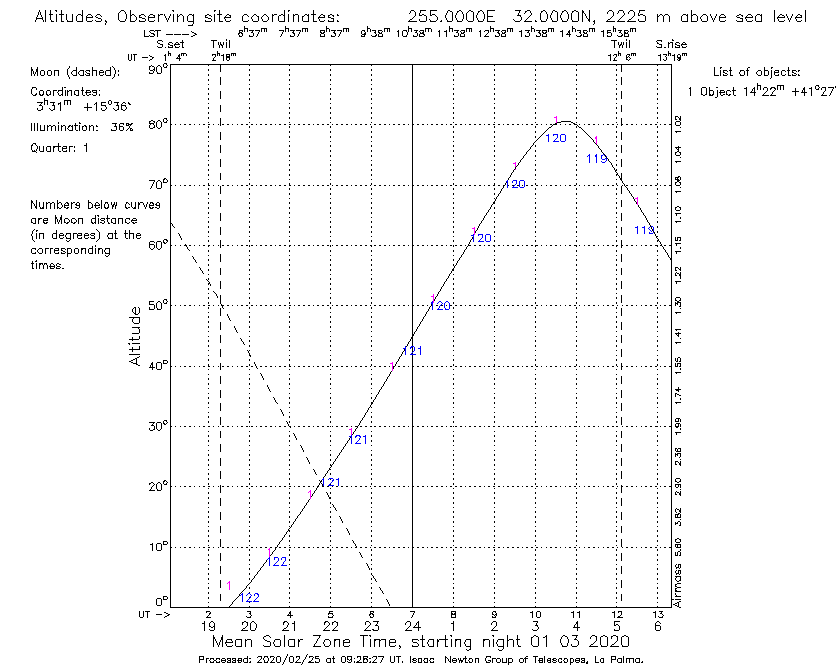
\includegraphics[width=0.5\textwidth]{1_3.PNG}&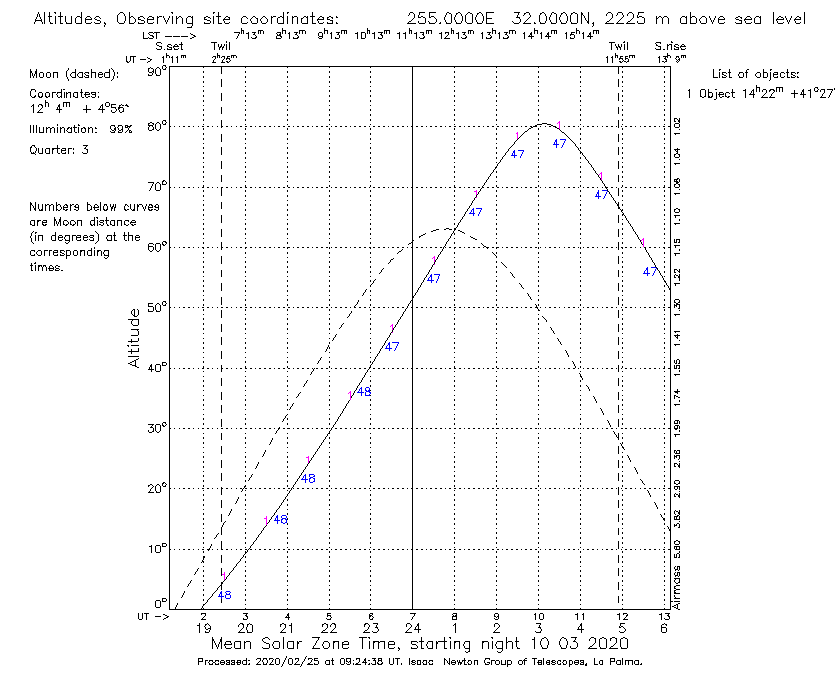
\includegraphics[width=0.5\textwidth]{10_3.PNG}  \\
    \end{tabular}
    \caption{Altitude de l'étoile DU BOO et de la Lune (en pointillés) dans la nuit du 1/03 et du 10/03}
    \end{figure}

    
\section{Éphémérides}\label{section:Ephémérides}
En allant sur le site de \href{https://www.aavso.org/vsx/index.php?view=detail.top&oid=4446}{l'AAVSO}, nous pouvons trouver toute les informations concernant notre étoile dont nous aurons besoin pour cette étude par "The international variable star index". Dans l'onglet 'Ephemeris' se trouve une liste de dates auxquelles l'étoile est dans sa phase de magnitude minimum. Nous allons nous baser sur ces dates pour fixer la phase 0. Voici une reconstitution par python de la courbe de magnitude V de notre étoile. Les données nous viennent du site de l'université de strasbourg \cite{site:cds}. 

Sur le premier graphique (a) les données sont tels qu'on les à reçue. Nous faisons ensuite varier la position de la phase 0.0 pour s'accorder avec les dates données par le site de l'AAVSO. Nous utiliserons donc la deuxième présentation des données par la suite (b). 

\begin{figure}[h!]
    \centering
    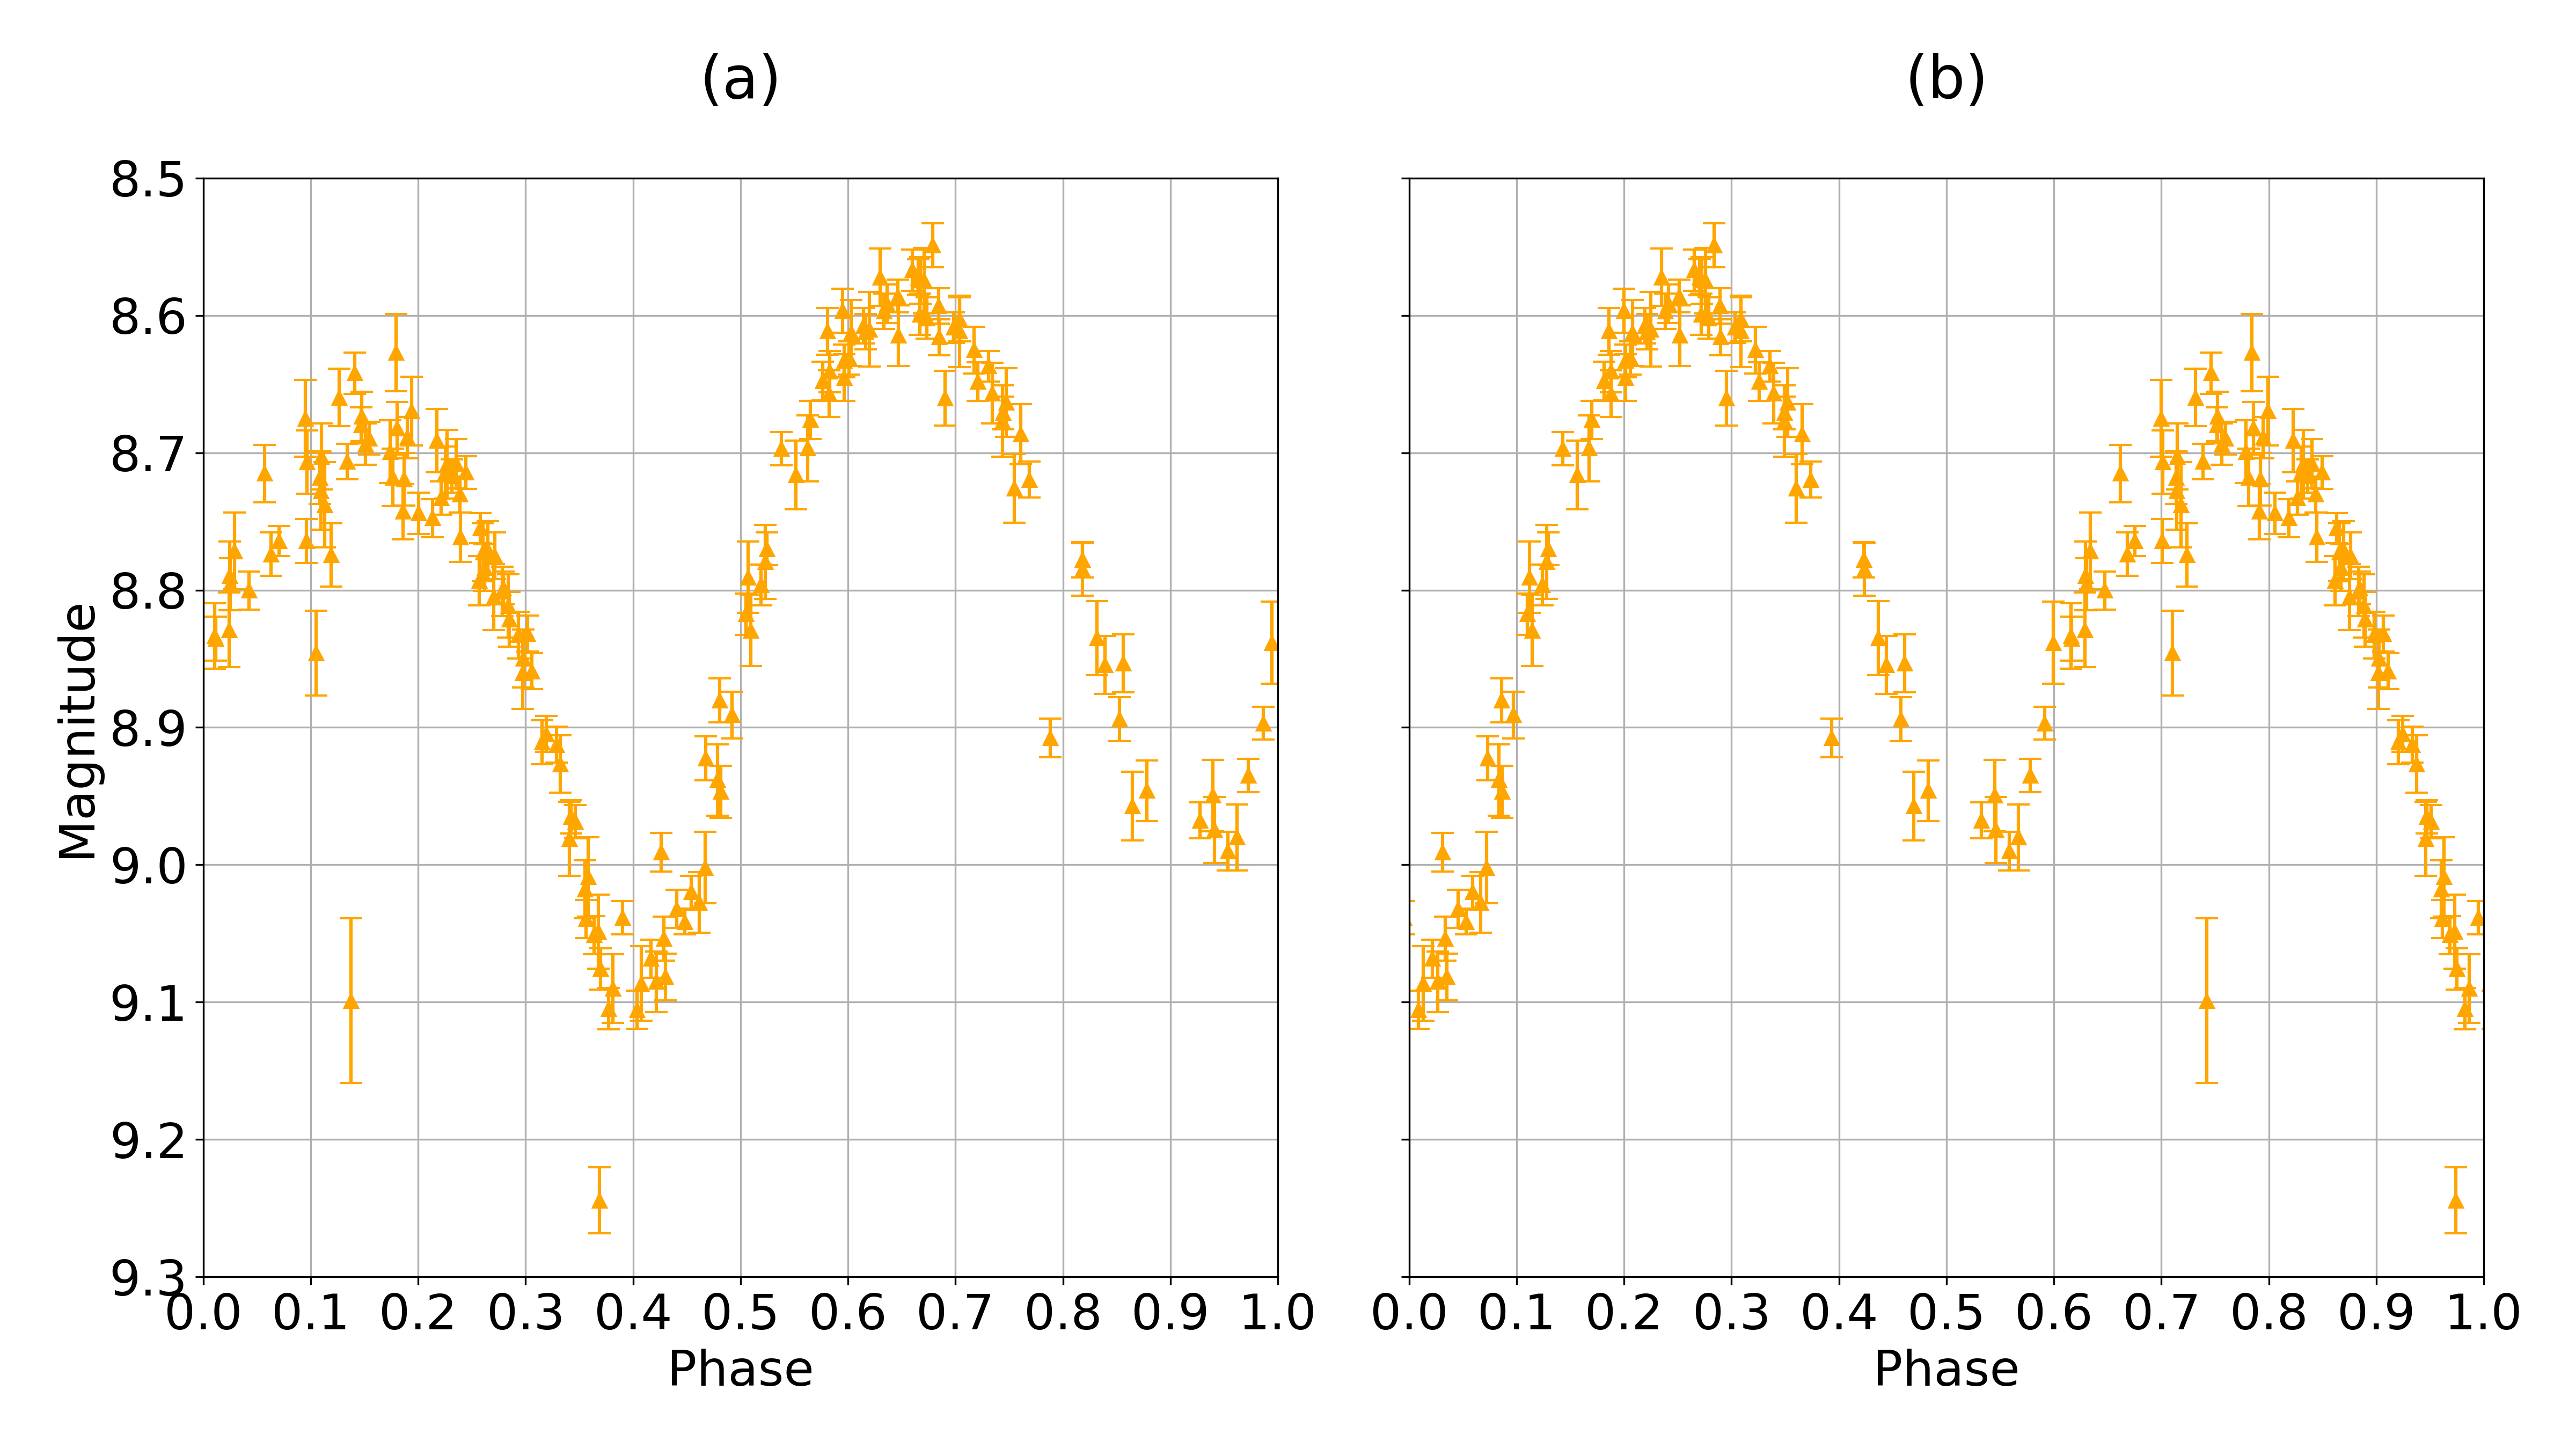
\includegraphics[width=0.5\textwidth]{cds_luminosite_centree.png}
    \caption{Variation de magnitude V en fonction de la phase}
    \label{fig:my_label}
\end{figure}

DU Boo est une étoile variable de type Beta Lyrae. La courbe de magnitude V est douce, c'est à dire sans pique ni plateau.Il semble intéressant de ne pas se concentrer uniquement sur ses extrema, contrairement au cas d'une binaire à éclipse qui présente des plateaux. Nous répartissons donc les 15 phases à observer de manière uniforme puis nous en varions certaines pour observer les maxima et minima de la courbe. Nous obtenons la distribution suivante :

\begin{figure}[h!]
    \centering
    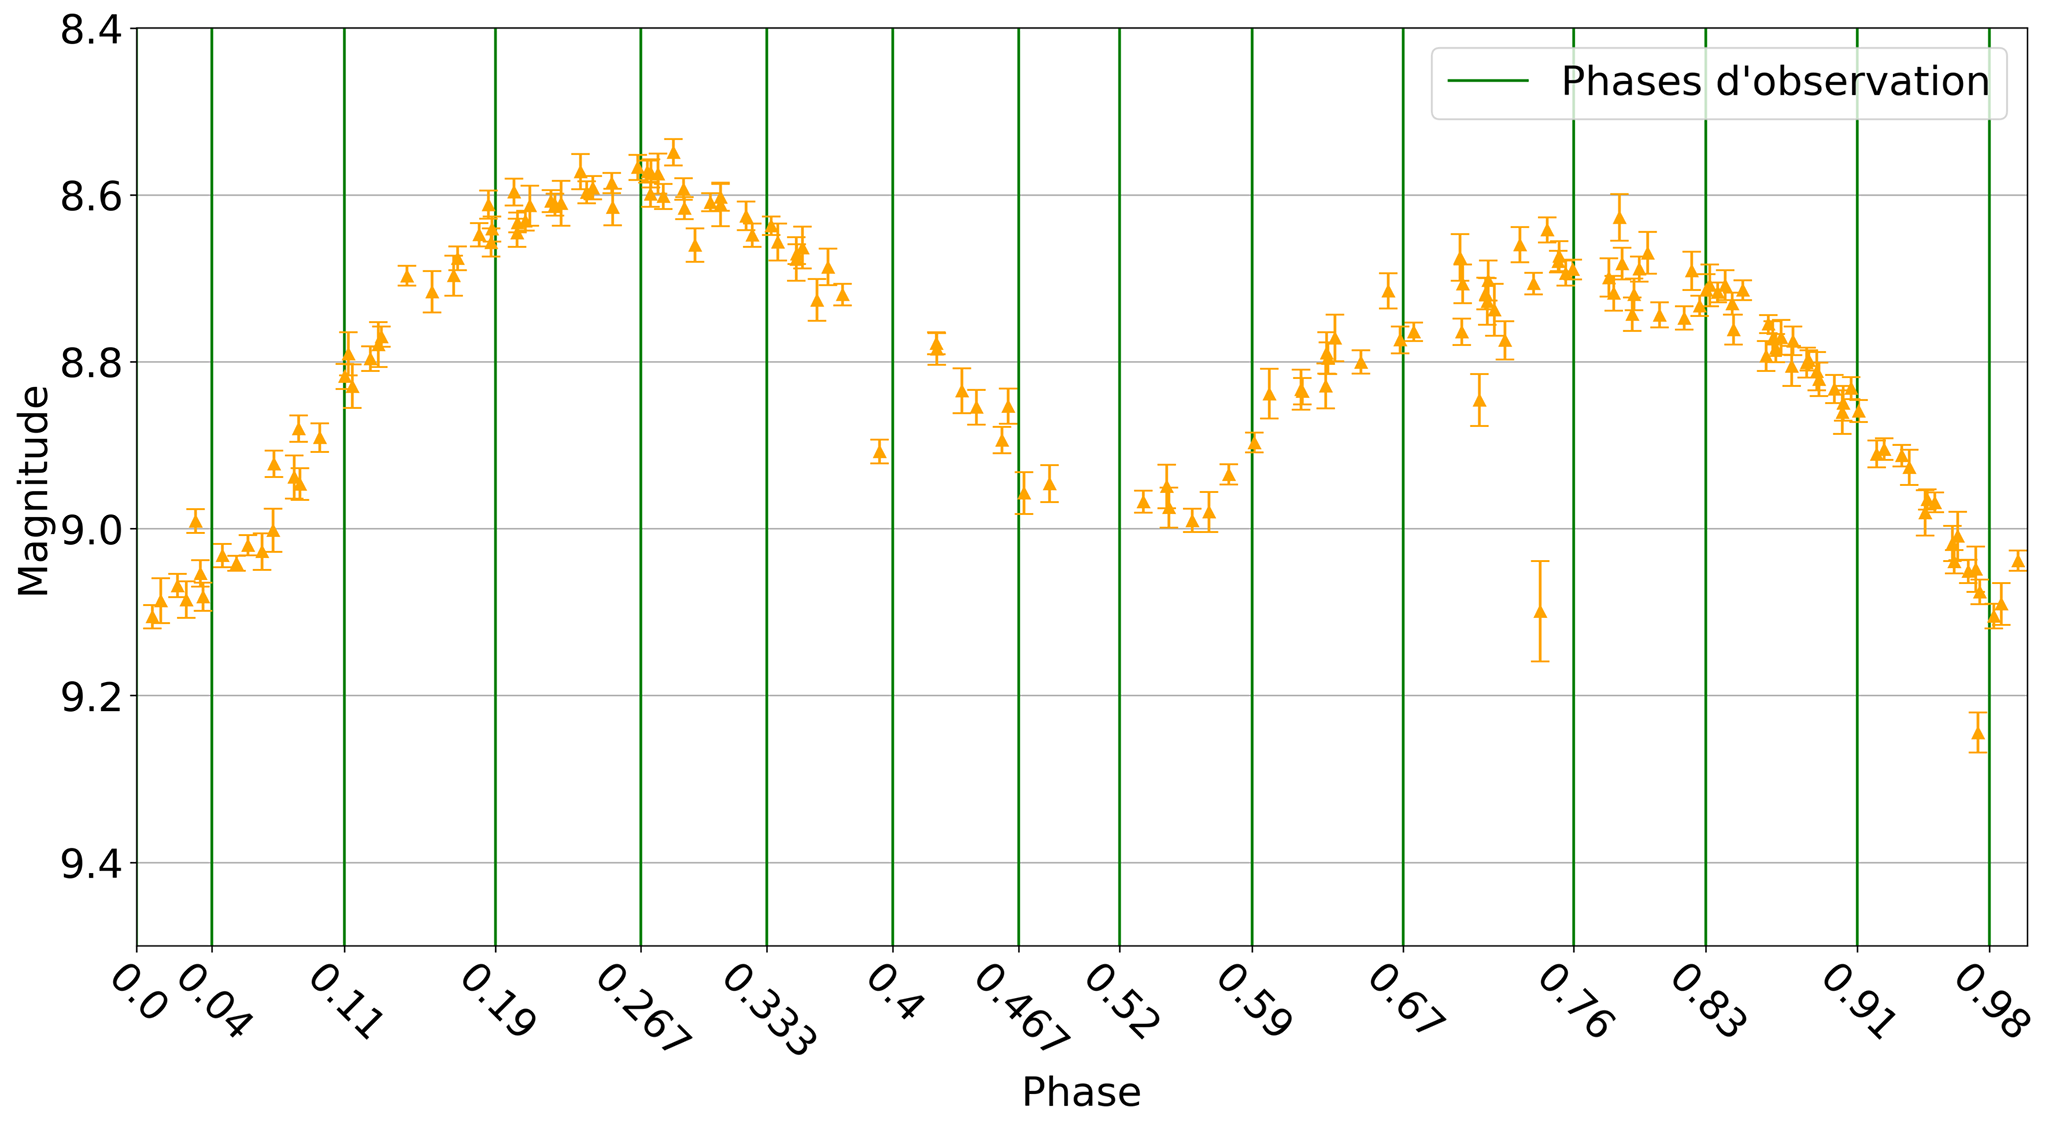
\includegraphics[width=0.5\textwidth]{Lumin+phase1.png}
    \caption{Distribution des phases à observer}
    \label{fig:my_label}
\end{figure}


\section{Détermination de l'étoile de comparaison}
    Une étoile de comparaison nous permet de mesurer la magnitude de notre étoile sur les clichés. Sur chaques clichés nous calculerons la magnitude relative de DU Boo par rapport à celle de l'étoile de comparaison et nous aurons ainsi une meilleure appréciation de la magnitude réelle de l'étoile. Évidemment la magnitude de l'étoile de comparaison doit être constante et elle doit être suffisamment proche de DU Boo pour apparaître sur le même cliché. Il est aussi important que sa magnitude soit semblable à celle de DU Boo ($\approx 8.7$) sans pour autant la dépasser car nous fixerons par la suite le temps de pose optimal par rapport à la magnitude maximale de DU Boo. 
    
    En utilisant Aladdin Lite nous pouvons voir les environs de notre étoile et évaluer quelles seraient les meilleurs étoiles de comparaison. Nous fixons notre choix sur les étoiles HD 126426 (V=8.76) et BD+42 2483 (V=9.06). Pour être sûr qu'elles se trouverons sur les photos prisent nous utilisons le site \href{https://telescopius.com/telescope-simulator}{Telescopius} qui détient déjà toute les caractéristique du télescope T5. Nous avons ainsi un aperçu des clichés que nous recevrons et nous pouvons déterminer les coordonnées les plus judicieuses à viser au télescope.  
    \begin{figure}[h!]
        \centering
        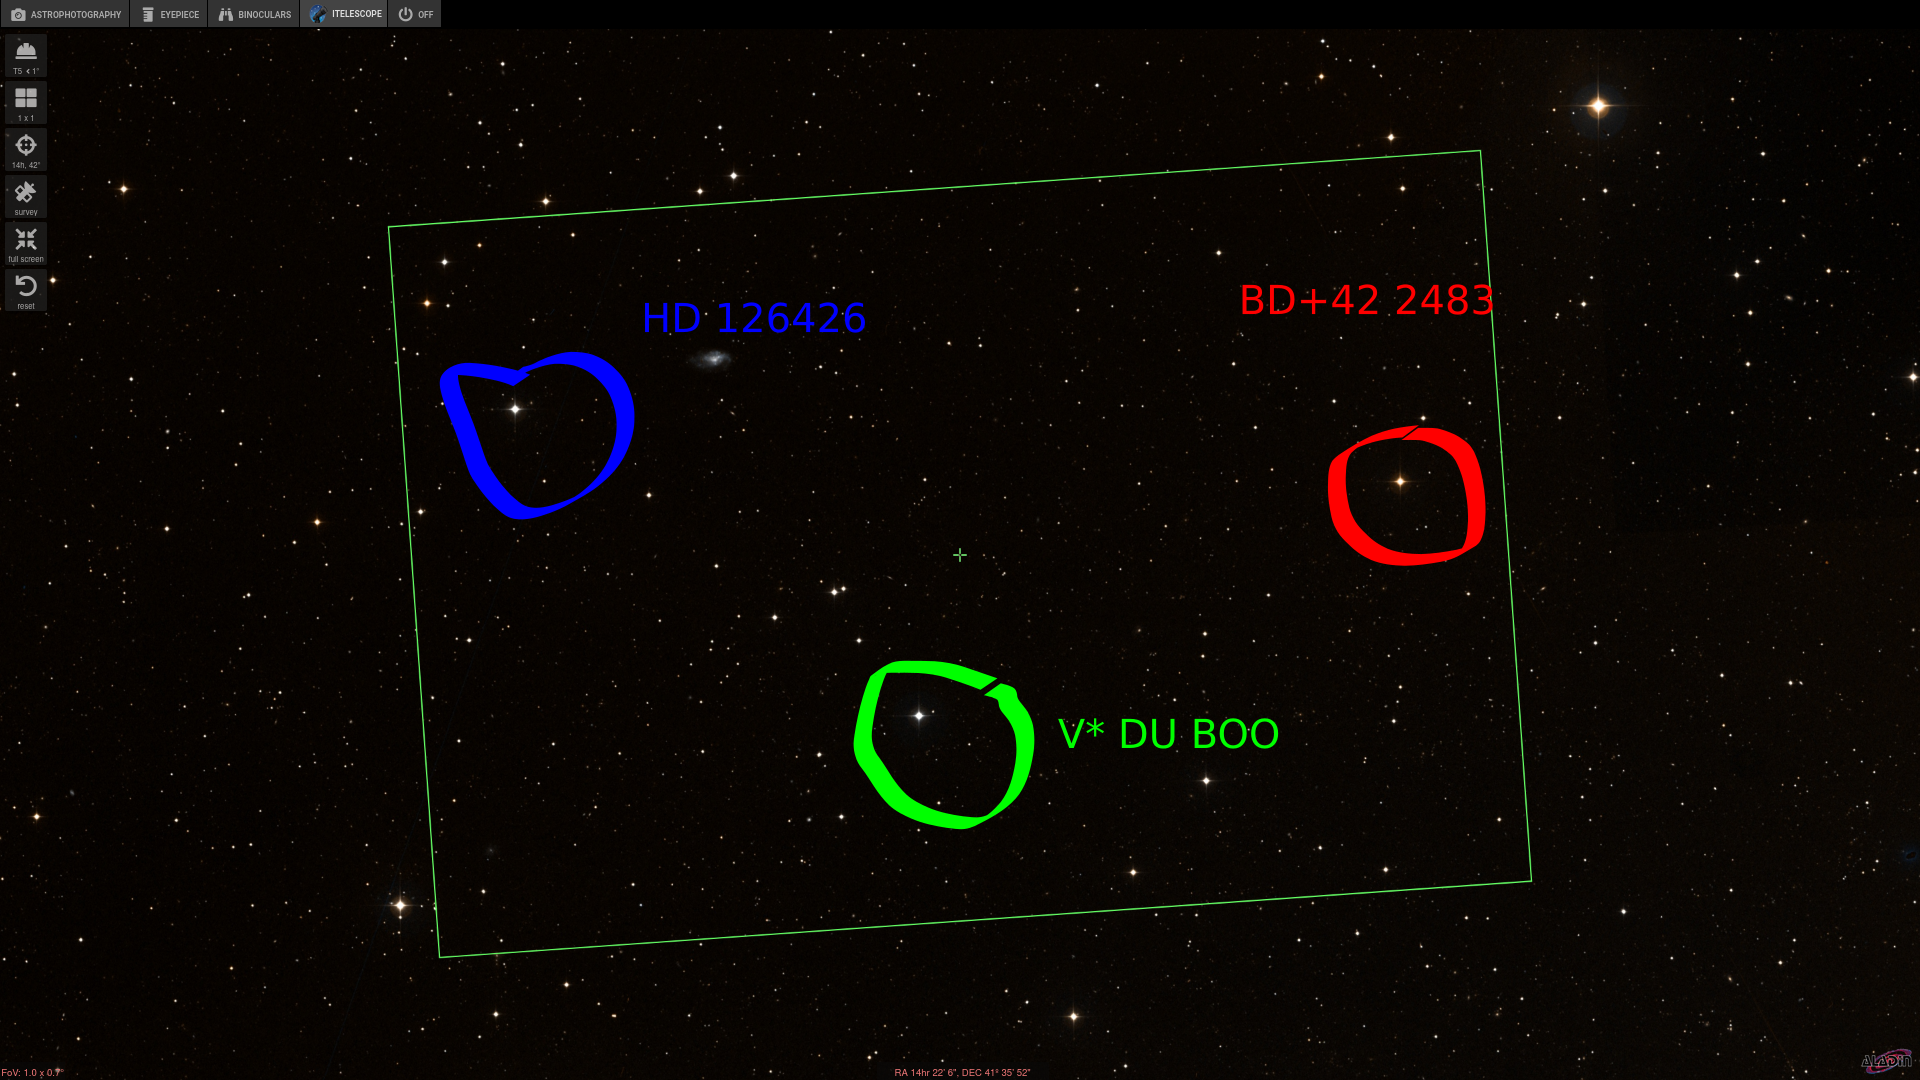
\includegraphics[width=0.4\textwidth]{telesco.png}
        \caption{Simulation des photos attendues avec localisation des étoiles d'intérêt}
        \label{fig:my_label}
    \end{figure}
    \newpage
    Nous allons donc prendre des photos centrées sur les coordonnées = 14hr22'6" 41\degree35'52" pour avoir sur nos clichés les trois étoiles d'intérêt.
\pagebreak
\section{Temps de pose optimal}

    Afin de déterminer la réponse du CCD en fonction du temps d'exposition, on utilise la série d'images de l'étoile HD 5505, de magnitude V = 9, mis à disposition \footnote{http://www.astro.ulb.ac.be/~siopis/hd-5505.zip}. Cette étoile est un standard photométrique, sa magnitude reste donc constante et est déterminée avec une grande précision \cite{notes}. On identifie d'abord l'étoile grâce à l'outil Aladin lite \footnote{https://aladin.u-strasbg.fr/AladinLite/} qui nous fournit une image du voisinage de HD 5505, et nous permet de remarquer que le télescope utilisé inverse l'image horizontalement. L'étoile est placée au centre de l'image. On peut maintenant procéder à l'analyse de sa photométrie, à l'aide du logiciel IRIS. Il existe deux méthodes de photométrie : PSF (Point Spread Function) et d'ouverture. La photométrie PSF procède à un ajustement d'une fonction gaussienne à deux dimensions sur l'étoile incluse dans la zone sélectionnée. L'intensité mesurée est alors l'intégrale de cette fonction gaussienne pour un sigma donné. La photométrie d'ouverture est une méthode plus directe, où le pointeur de la souris est remplacé par un cercle, que l'on centre sur l'étoile avant de cliquer. Le logiciel renvoie alors la somme des intensités de tous les pixels contenus dans ce cercle, qui est la somme du signal de l'étoile et du ciel. Il faut donc réitérer la procédure dans une partie vide du ciel afin d'obtenir la valeur de l'intensité du ciel à retirer à celle obtenue précédemment. La fonction de photométrie d'ouverture à deux cercles permet d'automatiser ces opérations, en retranchant la valeur médiane de l'intensité dans l'anneau composé par les deux cercles\footnote{le fait de prendre la valeur médiane et non moyenne permet d'éliminer partiellement des signaux parasites dus à des rayons cosmiques, étoiles à faible luminosité, etc..} à la somme des intensités mesurées dans le cercle extérieur. Une fonction à 3 cercles permet de rajouter une zone tampon entre celle utilisée pour la mesure de l'intensité du ciel, et le cercle intérieur où se trouve l'étoile afin de s'assurer que le signal de l'étoile ne vient pas perturber la mesure de l'intensité du ciel. La photométrie d'ouverture permet une mesure de haute précision si le ciel présente une faible densité d'étoiles. La photométrie PSF permet de mieux extraire le signal de l'étoile cible si le ciel présente un forte densité d'étoiles. Dans notre cas, il sera donc plus intéressant d'utiliser la photométrie d'ouverture, le ciel étant faiblement peuplé d'étoiles dans nos images.\cite{site:iris, inbook:warner:primer} 
    
    
    \begin{figure}[h!]
        \centering
        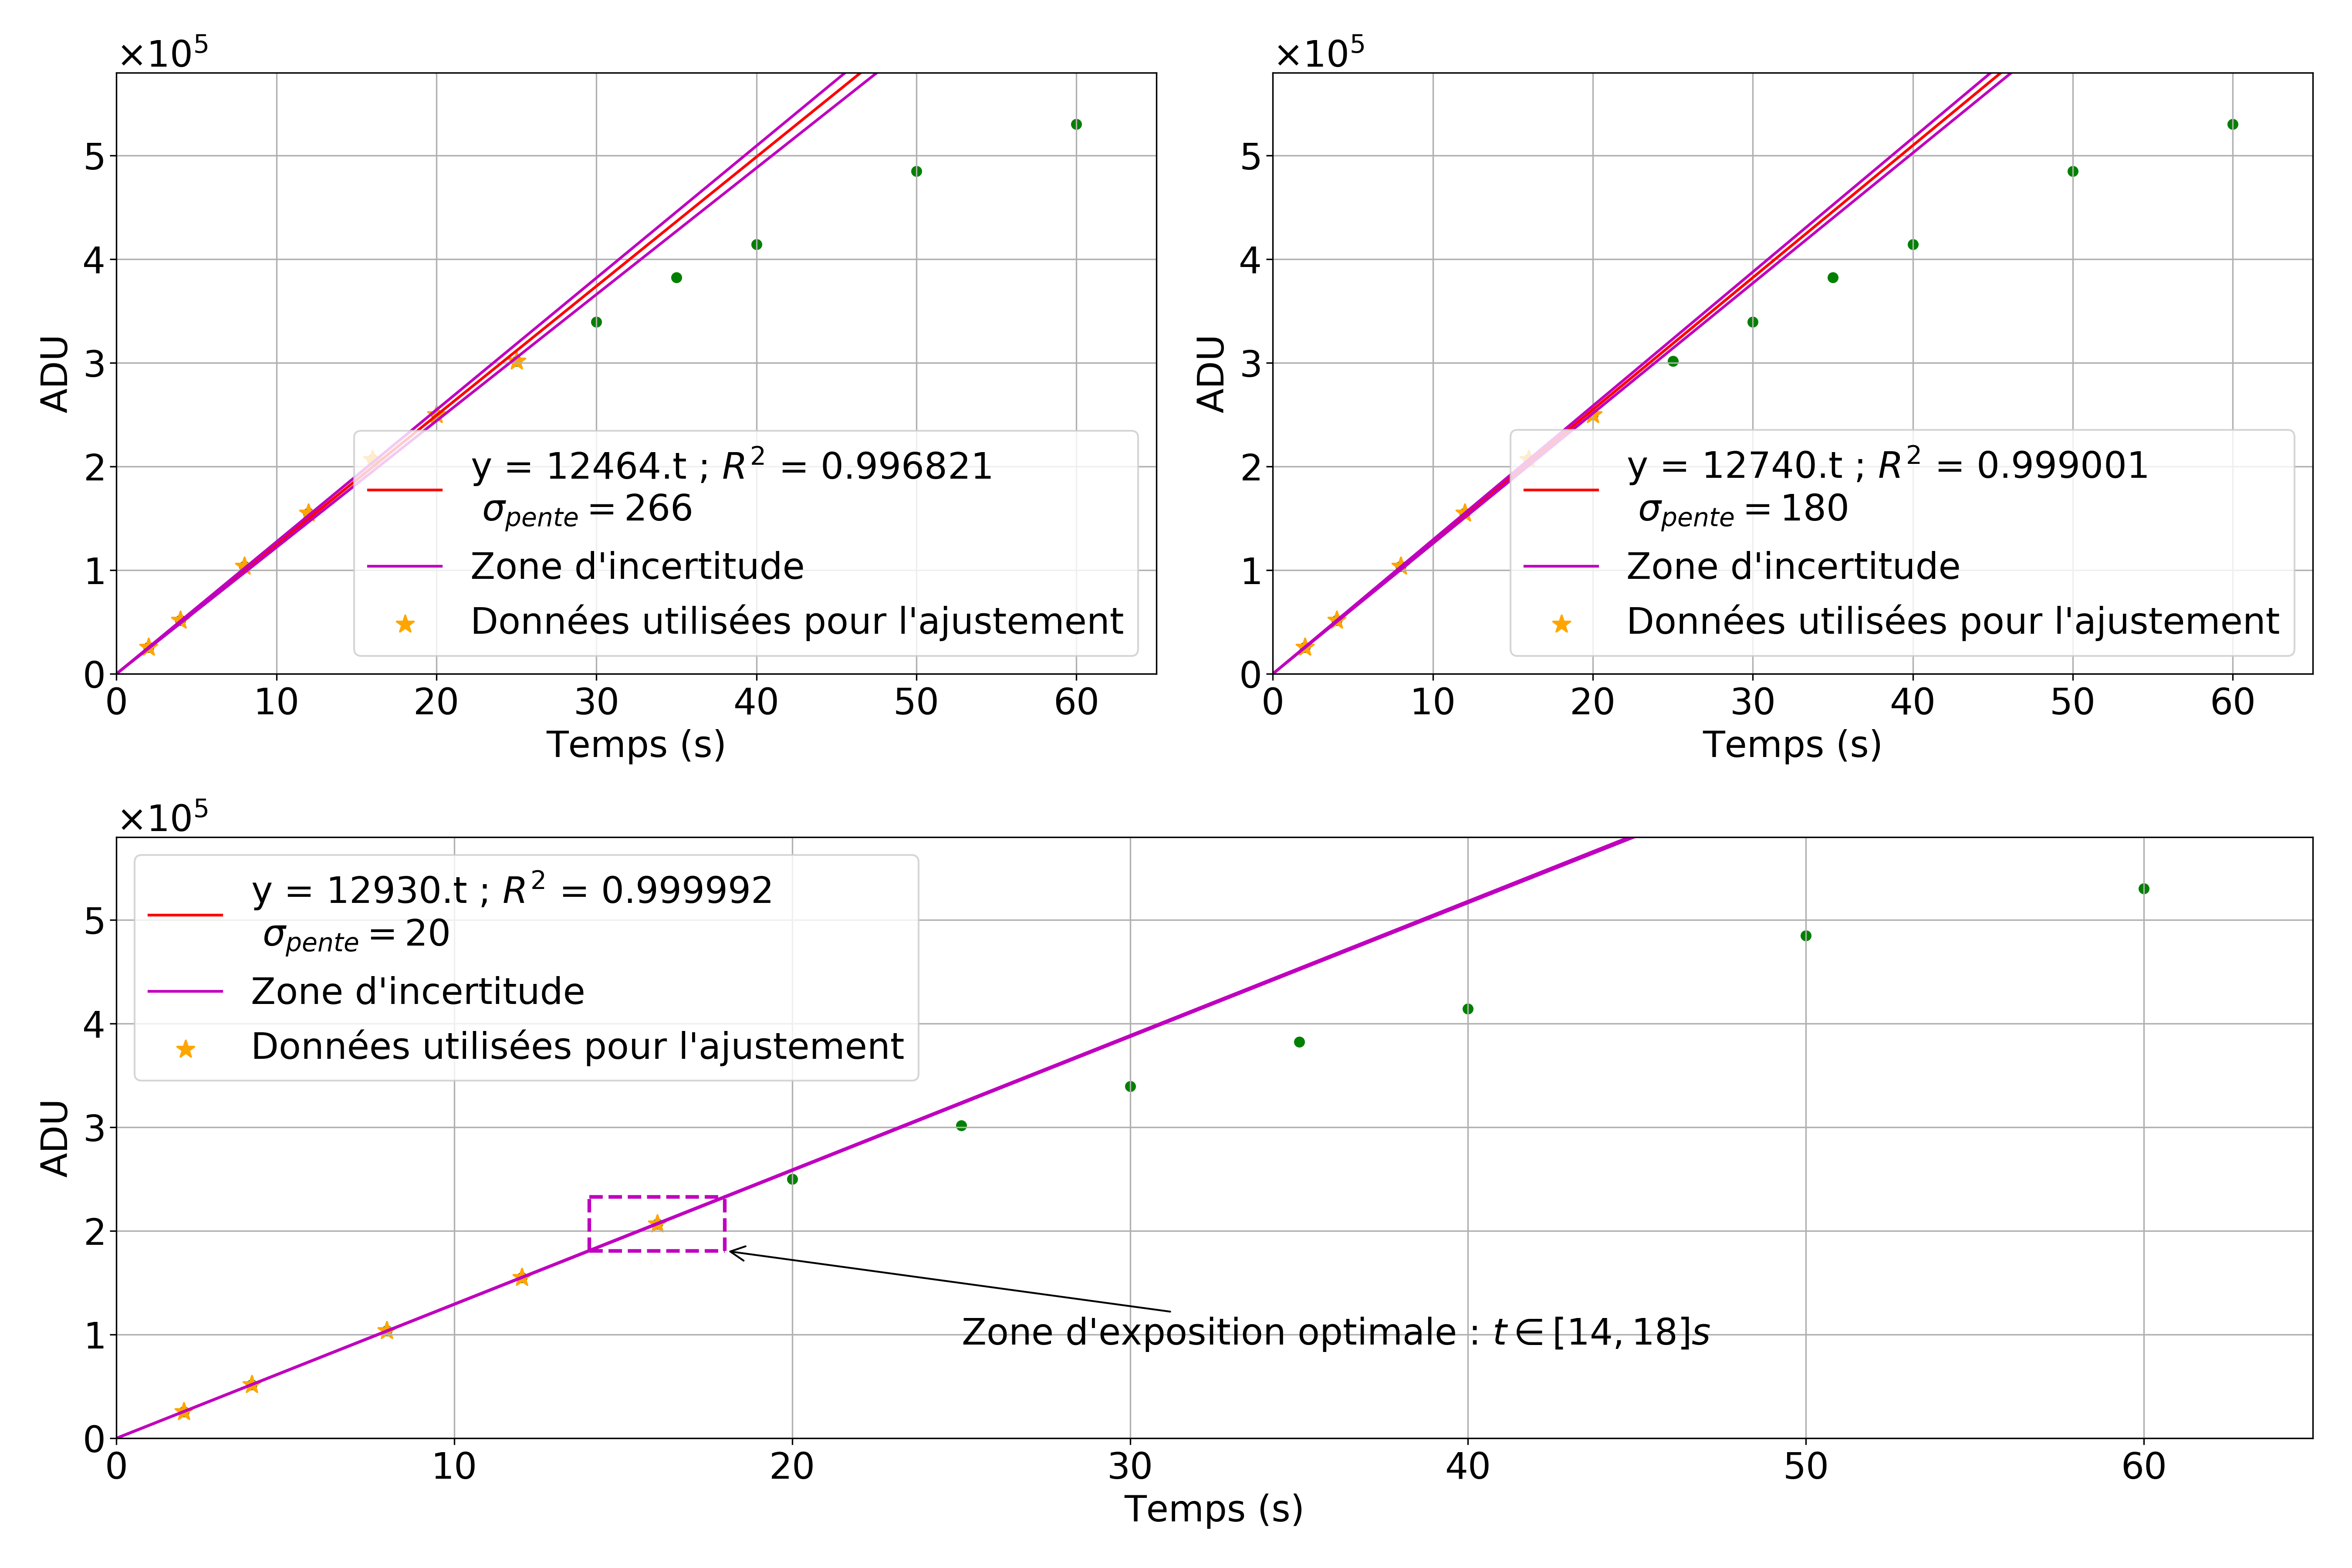
\includegraphics[width = \textwidth]{graph_temps_de_pose}
        \caption{Flux lumineux en fonction du temps pour l'étoile HD 5505 avec le télescope T5}
        \label{fig:graph_temps_de_pose}
    \end{figure}
    
    On effectue alors les mesures d'intensité pour chacunes des images et traçons un graphique de l'intensité (en ADU\footnote{Analog to Digital Units}) en fonction du temps. On observe que la réponse du CCD est linéaire jusqu'à un certain temps, puis la courbe tend à s'écraser. On souhaite effectuer nos mesures dans la zone de linéarité de la réponse du CCD car il serait difficile de comparer les flux lumineux mesurés de notre étoile et de l'étoile de comparaison, si l'on ne sait pas dans quel régime on se trouve. Aussi, afin d'avoir le meilleur rapport signal sur bruit, on souhaite se placer aux valeurs les plus hautes de flux lumineux enregistré dans la zone de linéarité. On va donc effectuer des régressions linéaires en sélectionnant un nombre différent de points, afin de voir laquelle minimise le coefficient de détermination ainsi que l'incertitude sur la pente. On force aussi l'ordonnée à l'origine, car il est évident que le flux lumineux enregistré pour un temps de pose nul doit être nul. On a alors le graphique présenté dans la figure \ref{fig:graph_temps_de_pose} qui reprend trois régressions linéaires. On observe que le premier points qui dévie réellement de la tendance linéaire est celui pour un temps de pose de 20s. La réponse du CCD cesse donc d'être linéaire entre un temps de pose de 16 secondes et de 20 secondes. Le temps de pose optimal doit donc se situer entre 14 et 18 secondes. On peut donc définir le temps d'exposition optimal pour HD 5505 avec ce télescope à 16 seconde, par prudence.

    Ceci fait, comment trouver le temps de pose optimal pour l'observation de notre étoile (de comparaison ou notre variable, selon laquelle atteindra la magnitude maximale que l'on observera), connaissant le temps de pose optimal pour l'étoile HD 5505 observé à travers un télescope de référence (ici T5), les magnitudes de HD 5505 et de notre étoile, ainsi que les diamètres du télescope de référence, et de celui que nous utiliserons.
    On considérera que les capteurs utilisés dans les deux télescopes ont la même réponse.
    
    On note :
    
    \begin{itemize}
    
        \item $t^{opt}_{HD}$ le temps d'exposition optimal pour HD 5505 avec le télescope de référence
        \item $t^{opt}_{Etoile}$ le temps d'exposition optimal pour notre étoile avec le télescope T5
        \item $E_{HD}^{ref}$ l'éclairement lumineux moyen de HD 5505 dans le télescope de référence
        \item $E_{Etoile}^{T5}$ l'éclairement lumineuxmoyen de notre étoile dans le télescope T5
        \item $E_{Etoile}^{ref}$ l'éclairement lumineux moyen de notre étoile dans le télescope de référence
        \item $D_{ref}$ le diamètre du télescope de référence
        \item $D_{T5}$ le diamètre du télescope T5
        
    \end{itemize}
    
    On cherche le temps de pose optimal, tel que la charge enregistrée en ADU pour notre étoile à travers T5 soit égale à celle enregistrée pour l'étoile HD 5505 à travers le télescope T5 pendant le temps $t^{opt}_{HD}$, afin de rester dans la région où la réponse du capteur reste linéaire. En d'autres termes, on cherche $t^{opt}_{Etoile}$ tel que :
    
    \begin{equation}
        \label{temps_de_pose}
        t^{opt}_{Etoile} \cdot E_{Etoile}^{T5} = t^{opt}_{HD} \cdot E_{HD}^{ref}
    \end{equation}
    
    Où l'on a que le flux reçu de notre étoile et le flux reçu de HD 5505 sont égaux.
    A partir des deux équations suivantes, on peut se ramener à des grandeurs connues \cite{site:wiki:magnitude, site:wiki:eclairement}:
    
    \begin{align}
        M_1 - M_2 &= - 2,5 log_{10}\left(\frac{E_1}{E_2}\right) \\
        E &= \frac{\Phi}{S}
    \end{align}
    
    Où $M$ représente la magnitude apparente de l'étoile, $\Phi$ le flux de lumière incident, et $S$ la surface éclairée. On considère ici que la surface éclairée correspond à la surface du miroir primaire du télescope. On peut donc réécrire l'équation \eqref{temps_de_pose} comme suit :
    
    \begin{align*}
        t^{opt}_{Etoile} \cdot \frac{\Phi_{Etoile}}{S_{T5}} &= t^{opt}_{HD} \cdot \frac{\Phi_{HD}}{S_{ref}} \\
        t^{opt}_{Etoile} \cdot \frac{4\Phi_{Etoile}}{\pi D_{T5}^2} &= t^{opt}_{HD} \cdot \frac{4\Phi_{HD}}{\pi D_{ref}^2} \\
        t^{opt}_{Etoile} &= t^{opt}_{HD} \cdot \frac{\Phi_{HD}}{\Phi_{Etoile}}\frac{D_{T5}^2}{D_{ref}^2} \\
        t^{opt}_{Etoile} &= t^{opt}_{HD} \cdot 10 ^{\left(\frac{M_{Etoile} - M_{HD}}{2,5}\right)} \left( \frac{D_{T5}}{D_{ref}} \right) ^2
    \end{align*}
    
    Dans notre cas ce résultat ce simplifie, car le télescope de référence utilisé n'est autre que T5. On a donc finalement, que le temps de pose optimal relatif à notre étoile est donné par :
    
    \begin{equation}
        t^{opt}_{Etoile} = t^{opt}_{HD} \cdot 10 ^{\left(\frac{M_{Etoile} - M_{HD}}{2,5}\right)}
    \end{equation}
    
    Ayant choisi une étoile de comparaison de magnitude inférieure à la magnitude maximale de DU BOO, nous prendrons donc comme valeur pour $M_{Etoile}$ la valeur maximale de la magnitude V de DU BOO. On trouve cependant plusieurs valeurs pour cette dernière. En effet, on trouve :
    
    \begin{itemize}
        \item Les valeurs données par le satellite Hipparcos nous donne une magnitude comprise entre 8,59 et 9,08, mais ce satellite était équipé d'un filtre spécifique. Cette magnitude est désignée sous l'appellation $H_p$, et bien que proche du spectre de la bande V, la bande $H_p$ diffère légèrement. Dans le catalogue Hipparcos, on trouve une valeur pour la magnitude V de 8,68, cependant il n'est indiqué si il s'agit de la magnitude maximale, minimale, moyenne ou médiane. La seule information sur cette magnitude est qu'elle provient des valeurs $V_T$ et $B_T$ de la photométrie Tycho, dont les gammes sont légèrement différentes des gammes V et B du système Johnson Cousins. On courbe présentée dans la section \ref{section:Ephémérides} reprend les données obtenues par ce satellite. \cite{article:hipp, site:hipp, site:hptransmission}
        \item Les valeurs relevées par le télescope OMC\footnote{Optical Monitoring Camera, à bord de la mission INTEGRAL lancé par l'ESA} place la magnitude V de notre étoile entre 8,54 et 9,03. La courbe de magnitude relevée par OMC est disponible \href{https://sdc.cab.inta-csic.es/omc/var/3038000045.html}{ici}\footnote{https://sdc.cab.inta-csic.es/omc/var/3038000045.html}\cite{article:iomc, article:catiomc}
        \item Les valeurs relevées par les équipes des observatoires de Stara Lesna (SL) et Skalnate Pleso de l'Institut Astronomique de l'Académie des Sciences Slovaque. Les magnitudes V sont comprises entre 8,60 et 9,08.\cite{article:catiaass}
    \end{itemize}
    
    On peut d'abord éliminer les valeurs obtenues par le satellite Hipparcos car ne correspondant pas à la gamme de lumière que nous allons observer. Les valeurs obtenues par OMC ont été mesurées hors atmosphère, il est donc logique que les magnitudes enregistrées soit légèrement supérieures à celles trouvées par les équipes des observatoires au sol. Comme nos observations vont s'effectuer au sol, nous utiliserons comme valeur de référence pour la magnitude V maximale, celle trouvée par l'Institut Astronomique de l'Académie des Sciences Slovaque, soit 8,60.
    On trouve alors que le temps de pose optimal est $t^{opt}_{Du BOO} = 11,07 s$.
\pagebreak    
\section{Calcul des dates d'observations}

    Maintenant que nous avons choisi le télescope que l'on va utiliser, ainsi que l'étoile que nous allons observer, tout en sachant que celle-ci sera observable pendant la période de fin-février -avril, il nous faut décider de dates d'observations.
    
    Avec les phases d'observations données plus haut, nous pouvons utiliser notre code, disponible sous sa version la plus récente \href{https://github.com/nicolasGrim/stage_astro/blob/master/Calcul\%20dates\%20d'observation\%20du\%20boo.ipynb}{au format jupyter notebook sur GitHub} \footnote{https://github.com/nicolasGrim/stage\_astro/blob/master/Calcul\%20dates\%20d'observation\%20du\%20boo.ipynb}, qui exploite les librairies astropy et astroplan sous python afin d'encoder les contraintes que l'on souhaite implémenter :
    
    \begin{itemize}
        \item L'observation doit se faire de nuit
        \item L'étoile doit être à une altitude supérieure à 30\degree en coordonnées horizontales afin d'être observable depuis l'observatoire et d'éviter une trop importante influence de la masse d'air \cite{site:T5, notes}
        \item L'étoile doit être à une distance angulaire supérieure à 30\degree de la lune, pour éviter une éventuelle pollution lumineuse.
    \end{itemize}
    
    L'utilisation de la librairie astroplan permet de réduire efficacement les lignes de codes à implémenter afin d'obtenir une liste de dates d'observations. Cependant, avant de découvrir l'existence de cette librairie, nous avons tenté deux approches :
    
    \begin{itemize}
        \item La première approche était un script python fonctionnel, mais peu optimisé, qui nous rendait une liste de dates d'observations possibles pour chacune des phases que l'on souhaitait observer, dont les heures étaient comprises entre 22h30 et 6h00. Cela permettait un premier tri quand aux dates possibles. Ensuite, l'idée était d'aller vérifier sur le module \href{http://catserver.ing.iac.es/staralt/}{STARALT du Isaac Newton Group} \footnote{http://catserver.ing.iac.es/staralt/} pour chacune des dates obtenues, l'altitude de notre étoile ainsi que sa distance angulaire avec la lune. On obtiendrait alors une liste de dates d'observations respectant les contraintes fixées. Il est à noter que le module STARALT nous permet aussi de vérifier que les dates d'observation choisies ont bien lieu pendant la nuit astronomique
        \item La deuxième approche fut d'utiliser certaines fonctions de la librairie astropy afin d'automatiser la procédure précédente. En effet, les fonction get\_moon() et get\_sun(), ainsi que Altaz permettent de trouver la position du soleil, ainsi que de la lune, en coordonnées horizontales depuis un lieu donné, et à un temps donné. Ainsi, il suffit de décider de ne garder que les dates pour lesquelles l'altitude du soleil est inférieure à -18\degree, ce qui nous garantit la nuit astronomique. Afin d'éviter toute pollution lumineuse de la part de la lune, il faut utiliser les coordonnées obtenues par la fonction get\_moon() et celles de notre étoile afin de calculer la distance angulaire entre les deux objets, et ne garder que les dates pour lesquelles cette dernière est inférieure à 30\degree. Enfin, le module Altaz permet d'obtenir l'altitude de notre étoile depuis l'observatoire, aux dates choisies, en coordonnées horizontales, ce qui nous permet de respecter la contrainte sur l'altitude.
    \end{itemize}
    
    Bien que ces approches fonctionnent, la lecture et l'utilisation du code utilisant la librairie astroplan sont bien plus aisées. Nous utiliserons donc ce code afin d'extraire les dates d'observations possibles, dont les premières sont présentées dans la table \ref{tab:dates_30}. Afin d'être certain de ne pas avoir fait d'erreur, on vérifie que les conditions soient respectées pour les dates choisies par l'intermédiaire du module STARALT. On voit sur la figure \ref{fig:staralt} l'altitude de notre étoile, et celle de la lune pour quelques-unes des dates renvoyées par notre code. Les conditions sont bien respectées\footnote{La distance angulaire à la lune sur la figure \ref{fig:staralt} est indiqué en bleu sous la courbe d'altitude de notre étoile.}. Bien que les dates et heures présentées dans cette figures respectent les conditions que nous avons fixées, on remarque cependant que l'altitude de l'étoile est loin de son maximum. En effet celle-ci 
           \begin{wraptable}{l}{0.65\textwidth}
    
            \centering
            
            \begin{tabular}{|l|l|l|l|}
                \toprule
                {}Phase&                    1 &                    2 &                    3 \\
                \midrule
                0.000 &  24 févr. $04{:}55{:}30$ &   08 mars $22{:}21{:}44$ &   09 mars $23{:}42{:}13$ \\
                0.040 &   08 mars $23{:}22{:}33$ &   10 mars $00{:}43{:}02$ &   11 mars $02{:}03{:}31$ \\
                0.110 &   06 mars $22{:}28{:}02$ &   07 mars $23{:}48{:}30$ &   09 mars $01{:}08{:}59$ \\
                0.190 &   05 mars $23{:}09{:}11$ &   07 mars $00{:}29{:}40$ &   08 mars $01{:}50{:}09$ \\
                0.267 &   04 mars $23{:}45{:}17$ &   06 mars $01{:}05{:}45$ &   07 mars $02{:}26{:}14$ \\
                0.333 &   02 mars $22{:}45{:}41$ &   04 mars $00{:}06{:}10$ &   05 mars $01{:}26{:}39$ \\
                0.400 &   01 mars $23{:}06{:}34$ &   03 mars $00{:}27{:}03$ &   04 mars $01{:}47{:}32$ \\
                0.467 &  29 févr. $23{:}27{:}27$ &   02 mars $00{:}47{:}56$ &   03 mars $02{:}08{:}25$ \\
                0.520 &  28 févr. $23{:}28{:}04$ &   01 mars $00{:}48{:}33$ &   02 mars $02{:}09{:}02$ \\
                0.590 &  27 févr. $23{:}54{:}01$ &  29 févr. $01{:}14{:}30$ &   01 mars $02{:}34{:}59$ \\
                0.670 &  25 févr. $23{:}14{:}42$ &  27 févr. $00{:}35{:}11$ &  28 févr. $01{:}55{:}40$ \\
                0.760 &  25 févr. $00{:}11{:}04$ &  26 févr. $01{:}31{:}33$ &  27 févr. $02{:}52{:}02$ \\
                0.830 &  25 févr. $01{:}57{:}30$ &  26 févr. $03{:}17{:}59$ &  27 févr. $04{:}38{:}28$ \\
                0.910 &  25 févr. $03{:}59{:}08$ &   10 mars $22{:}45{:}51$ &   12 mars $00{:}06{:}20$ \\
                0.980 &   09 mars $23{:}11{:}48$ &   11 mars $00{:}32{:}17$ &   12 mars $01{:}52{:}46$ \\
                \bottomrule
            \end{tabular}

            \caption{Premières dates d'observation possibles (année 2020). La première colonne indique la phase. Les heures sont au fuseau horaire UTC - 7}
            
            \label{tab:dates_30}
        \end{wraptable}atteint son maximum entre 3h et 4h du matin pendant cette période. Plus l'étoile est proche du zénith et moins on aura de perturbations dues à la couche d'atmosphère traversée par la lumière. Comme la liste de dates retournée pour une altitude minimale de 30\degree est assez grande, nous pouvons choisir en priorité les dates pour lesquelles l'altitude de l'étoile est supérieure à 70\degree. On obtient alors la sélection de dates listées dans la table \ref{tab:dates_obs}, qui tient compte du fait que nous sommes limités à une observation par jour sur la plateforme iTelescope.\footnote{Pour consulter davantage de dates d'observations, se référer au notebook disponible sur GitHub}
        
        Une fois les dates d'observations déterminées, et le temps de pose optimal calculé, nous pouvons définir les OB (Observing Blocks). Le temps de réservation minimum étant de 15 minutes, nous choisissons de démarrer nos OB un minimum de 5 minutes avant la date choisie, et d'occuper le télescope pendant toute cette durée : On réalise 52 clichés avec des temps d'expositions de 11,07 secondes. Il faut rajouter à ce temps total 50\% du fait des différentes opérations que le télescope effectue entre deux clichés, ce qui nous donne un total d'un peu moins de 15 minutes. Nous sommes alors certain d'avoir au moins un cliché correspondant à la date voulue, et si nous le souhaitons, nous pourrons utiliser les autres afin d'augmenter le signal enregistré en superposant les images.
        
        \begin{table}[H]
        
            \centering
                        
            \begin{tabular}{|c|c|}
                \toprule
                 Phase &      Date d’observation \\
                \midrule
                 0.000 &  12 mars $02{:}23{:}10$ \\
                 0.040 &  11 mars $02{:}03{:}31$ \\
                 0.110 &  10 mars $02{:}29{:}28$ \\
                 0.190 &  08 mars $01{:}50{:}09$ \\
                 0.267 &  07 mars $02{:}26{:}14$ \\
                 0.333 &  06 mars $02{:}47{:}07$ \\
                 0.400 &  05 mars $03{:}08{:}00$ \\
                 0.467 &  04 mars $03{:}28{:}54$ \\
                 0.520 &  03 mars $03{:}29{:}30$ \\
                 0.590 &  02 mars $03{:}55{:}28$ \\
                 0.670 &  01 mars $04{:}36{:}37$ \\
                 0.760 &  16 mars $01{:}40{:}10$ \\
                 0.830 &  15 mars $02{:}06{:}08$ \\
                 0.910 &  14 mars $02{:}47{:}17$ \\
                 0.980 &  13 mars $03{:}13{:}14$ \\
                \bottomrule
            \end{tabular}
            \caption{Dates d'observation choisies pour les différentes phases}
            \label{tab:dates_obs}
        \end{table} 
        
        \begin{figure}[t]
        
            \centering
            
                \subfloat[2020-03-08 22:21:44]{\includegraphics[width=0.45\textwidth]{03-08}}
                \subfloat[2020-03-07 23:48:30]{\includegraphics[width=0.45\textwidth]{03-07}} \\
                \subfloat[2020-03-06 01:05:45]{\includegraphics[width=0.45\textwidth]{03-06}} 
                \subfloat[2020-03-05 23:09:11]{\includegraphics[width=0.45\textwidth]{03-05}} \\
                \subfloat[2020-03-04 23:45:16]{\includegraphics[width=0.45\textwidth]{03-04}} 
                \subfloat[2020-03-02 22:45:41]{\includegraphics[width=0.45\textwidth]{03-02}} \\
                
            \caption{Altitude de l'étoile DU BOO et de la lune (en pointillés) pour des dates obtenues par l'intermédiaire de notre code}
            
            \label{fig:staralt}
            
        \end{figure}
\chapter{Acquisition et analyse des données}\label{chapt:doe}

\section{Acquisition des données}
Après s'être familiarisé avec le site d'Itelescope, nous avons pu programmer notre première prise de donnée dans la nuit du 29 février au 1er mars. Après avoir confirmé avec nos maitre de stage que la procédure de réservation avait été réalisé correctement nous avons pu créer un calendrier de prise de mesure. Le tableau ci-dessous présente nos programmations jusqu'au 13 mars et si une photo a pu été prise ou non. 

\begin{figure}[h!]
    \centering
    \begin{tabular}{|c|c|c|c|}\hline
     Date ITelescope & Date locale & Phase et heure d'observation & Résultat \\ \hhline{|=|=|=|=|}
     29/02 & 01/03 & 0.670 à 4h36 & Mauvaise météo \\ \hline
     01/03 & 02/03 & 0.590 à 3h55 & Mauvaise météo\\ \hline
     03/03 & 04/03 & 0.520 à 4h49 & Mauvaise météo\\ \hline
     04/03 & 05/03 & 0.400 à 3h08 & Observation réussie\\ \hline
     05/03 & 05/03 & 0.190 à 23h09 & Observation réussie \\ \hline
     06/03 & 07/03 & 0.333 à 4h07 & Observation réussie\\ \hline
     07/03 & 08/03 & 0.267 à 3h46 & Mauvaise météo\\ \hline
     08/03 & 08/03 & 0.0 à 22h21 & Mauvaise météo\\ \hline
     09/03 & 10/03 & 0.040 à 0h43 & Mauvaise météo\\ \hline
     10/03 & 11/03 & 0.110 à 3h49 & Mauvaise météo\\ \hline
     11/03 & 12/03 & 0.980 à 1h52 & Mauvaise météo\\ \hline
     12/03 & 13/03 & 0.910 à 1h26 & Mauvaise météo\\ \hline
     13/03 & 14/03 & 0.830 à 0h45 & Erreur de changement d'heure et de cadrage\\ \hline
    \end{tabular}
    \caption{Première planification de prise de mesure}
    \label{fig:my_label}
\end{figure}

Tout ne s'est pas passé comme prévu. Tout d'abord nous pouvons constater que la météo du début du mois de mars n'est pas la meilleur. Beaucoup de nos observation n'ont pas pu se faire à cause de celle-ci. Ensuite, lors de la mesure du 13 mars nous n'avions pas pris en compte le changement d'heure au Nouveau Mexique. Nous avons donc déterminé que la photo prise avec un décalage de 1h correspondait à la phase 0.79 qui ne se trouve pas dans nos phases d'intérêts. Nous avons donc réarrangé nos phases pour qu'elles soient réparties de manières uniforme en considérant les 3 phases déjà mesurées les nuits du 4,5 et 6 mars et la phase 0.79. Nous avons décider de continuer nos mesures sur ces phases :

\newpage
\begin{figure}[h!]
    \centering
    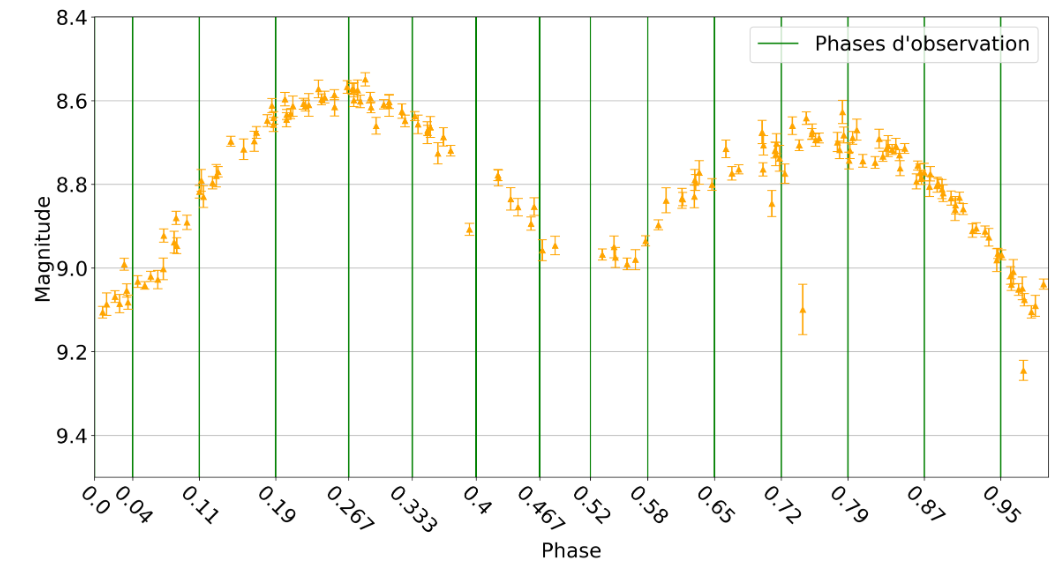
\includegraphics[width=0.4\textwidth]{Lumin+phase2.png}
    \caption{Nouvelle distribution des phases à observer}
    \label{fig:my_label}
\end{figure}

Nous avons alors reconstruit un calendrier de mesure en prenant en compte le changement d'heure du Nouveau Mexique et les nouvelles phases choisies. 

\begin{figure}[h!]
    \centering
    \begin{tabular}{|c|c|c|c|}\hline
     Date ITelescope & Date locale & Phase et heure d'observation & Résultat \\ \hhline{|=|=|=|=|}
     14/03 & 15/03 & 0.910 à 4h06 & Mauvais cadrage \\ \hline
     16/03 & 17/03 & 0.790 à 4h50 & Observation réussie\\ \hline
     18/03 & 19/03 & 0.650 à 3h54 & Mauvaise météo\\ \hline
     19/03 & 20/03 & 0.580 à 3h28 & Observation réussie\\ \hline
     20/03 & 21/03 & 0.520 à 2h17 & Mauvaise météo \\ \hline
     21/03 & 22/03 & 0.467 à 3h17 & Observation réussie\\ \hline
     22/03 & 22/03 & 0.267 à 23h33 & Mauvaise météo\\ \hline
     24/03 & 24/03 & 0.110 à 22h16 & Observation réussie\\ \hline
     26/03 & 26/03 & 0.040 à 23h10 & Mauvaise météo\\ \hline
     27/03 & 27/03 & 0.000 à 23h30 & Mauvaise météo\\ \hline
     28/03 & 28/03 & 0.950 à 23h34 & Observation réussie\\ \hline
     29/03 & 29/03 & 0.870 à 22h53 & Mauvaise météo\\ \hline
     30/03 & 31/03 & 0.040 à 4h32 & Observatin réussie\\ \hline
     31/03 & 31/03 & 0.720 à 21h46 & Mauvaise météo\\ \hline
    \end{tabular}
    \caption{Deuxième planification des prises de mesures}
    \label{fig:my_label}
\end{figure}

Après avoir obtenus la mesure du 14/03 nous avons analysé les photos obtenues ces derniers jours et nous nous sommes rendu compte que la photo du 13/03 et du 14/03 ne sont pas du tout bien cadré. Après échange sur la question avec nos maître de stage, nous pensons que c'est une erreur informatique de la part de ITelescope. Ces clichés sont donc inutilisable pour notre études vu que notre étoiles n'est pas présente sur les photos. 

A la fin du mois de mars nous avons 9 prise de mesure réussie sur les 27 essais. Ce n'est pas un taux très élevé. Mais on pouvait s'attendre à ce que la météo de fin d'hiver ne soit pas la plus optimale pour photographier les étoiles. On voit bien d'ailleurs que pour la deuxième partie du mois de mars la météo est bien moins handicapante pour la prise de donnée.

Début avril, les deux autres groupe réalisant le même stage que nous en sont arrivé au stade de prise de mesure et nous devons nous partager le même compte. Comme une seule prise de mesure est autorisé par nuit, nous décidons d'avancer dans la réalisation du stage avec ces 9 mesures. Une fois que les autres groupes auront obtenu un nombre suffisant de clichés exploitable, nous reprendrons quelques mesure pour tenter de compléter un maximum notre courbe de magnitude V.

\section{Analyse des données}
    \subsection{Stacking}
    \subsection{Correction des méta-données}
    \subsection{Photométrie d'ouverture avec Iris}
    \subsection{Photométrie de segmentation avec Photutils}
\chapter{Résultats}\label{chapt:model}

\pagebreak

\printbibheading[heading=bibintoc,title={Bibliographie}]
\printbibliography[type=inbook,heading=subbibliography,title={Livres}]
\printbibliography[type=book,heading=subbibliography,title={Livres}]
\printbibliography[type=article,heading=subbibliography,title={Articles}]
\printbibliography[type=online,heading=subbibliography,title={Sites internet}]
\printbibliography[nottype=book, nottype = inbook, nottype = article, nottype = online,heading=subbibliography,title={Autres sources}]
\end{document}
